% Options for packages loaded elsewhere
\PassOptionsToPackage{unicode}{hyperref}
\PassOptionsToPackage{hyphens}{url}
\documentclass[
]{article}
\usepackage{xcolor}
\usepackage[margin=1in]{geometry}
\usepackage{amsmath,amssymb}
\setcounter{secnumdepth}{-\maxdimen} % remove section numbering
\usepackage{iftex}
\ifPDFTeX
  \usepackage[T1]{fontenc}
  \usepackage[utf8]{inputenc}
  \usepackage{textcomp} % provide euro and other symbols
\else % if luatex or xetex
  \usepackage{unicode-math} % this also loads fontspec
  \defaultfontfeatures{Scale=MatchLowercase}
  \defaultfontfeatures[\rmfamily]{Ligatures=TeX,Scale=1}
\fi
\usepackage{lmodern}
\ifPDFTeX\else
  % xetex/luatex font selection
\fi
% Use upquote if available, for straight quotes in verbatim environments
\IfFileExists{upquote.sty}{\usepackage{upquote}}{}
\IfFileExists{microtype.sty}{% use microtype if available
  \usepackage[]{microtype}
  \UseMicrotypeSet[protrusion]{basicmath} % disable protrusion for tt fonts
}{}
\makeatletter
\@ifundefined{KOMAClassName}{% if non-KOMA class
  \IfFileExists{parskip.sty}{%
    \usepackage{parskip}
  }{% else
    \setlength{\parindent}{0pt}
    \setlength{\parskip}{6pt plus 2pt minus 1pt}}
}{% if KOMA class
  \KOMAoptions{parskip=half}}
\makeatother
\usepackage{color}
\usepackage{fancyvrb}
\newcommand{\VerbBar}{|}
\newcommand{\VERB}{\Verb[commandchars=\\\{\}]}
\DefineVerbatimEnvironment{Highlighting}{Verbatim}{commandchars=\\\{\}}
% Add ',fontsize=\small' for more characters per line
\usepackage{framed}
\definecolor{shadecolor}{RGB}{248,248,248}
\newenvironment{Shaded}{\begin{snugshade}}{\end{snugshade}}
\newcommand{\AlertTok}[1]{\textcolor[rgb]{0.94,0.16,0.16}{#1}}
\newcommand{\AnnotationTok}[1]{\textcolor[rgb]{0.56,0.35,0.01}{\textbf{\textit{#1}}}}
\newcommand{\AttributeTok}[1]{\textcolor[rgb]{0.13,0.29,0.53}{#1}}
\newcommand{\BaseNTok}[1]{\textcolor[rgb]{0.00,0.00,0.81}{#1}}
\newcommand{\BuiltInTok}[1]{#1}
\newcommand{\CharTok}[1]{\textcolor[rgb]{0.31,0.60,0.02}{#1}}
\newcommand{\CommentTok}[1]{\textcolor[rgb]{0.56,0.35,0.01}{\textit{#1}}}
\newcommand{\CommentVarTok}[1]{\textcolor[rgb]{0.56,0.35,0.01}{\textbf{\textit{#1}}}}
\newcommand{\ConstantTok}[1]{\textcolor[rgb]{0.56,0.35,0.01}{#1}}
\newcommand{\ControlFlowTok}[1]{\textcolor[rgb]{0.13,0.29,0.53}{\textbf{#1}}}
\newcommand{\DataTypeTok}[1]{\textcolor[rgb]{0.13,0.29,0.53}{#1}}
\newcommand{\DecValTok}[1]{\textcolor[rgb]{0.00,0.00,0.81}{#1}}
\newcommand{\DocumentationTok}[1]{\textcolor[rgb]{0.56,0.35,0.01}{\textbf{\textit{#1}}}}
\newcommand{\ErrorTok}[1]{\textcolor[rgb]{0.64,0.00,0.00}{\textbf{#1}}}
\newcommand{\ExtensionTok}[1]{#1}
\newcommand{\FloatTok}[1]{\textcolor[rgb]{0.00,0.00,0.81}{#1}}
\newcommand{\FunctionTok}[1]{\textcolor[rgb]{0.13,0.29,0.53}{\textbf{#1}}}
\newcommand{\ImportTok}[1]{#1}
\newcommand{\InformationTok}[1]{\textcolor[rgb]{0.56,0.35,0.01}{\textbf{\textit{#1}}}}
\newcommand{\KeywordTok}[1]{\textcolor[rgb]{0.13,0.29,0.53}{\textbf{#1}}}
\newcommand{\NormalTok}[1]{#1}
\newcommand{\OperatorTok}[1]{\textcolor[rgb]{0.81,0.36,0.00}{\textbf{#1}}}
\newcommand{\OtherTok}[1]{\textcolor[rgb]{0.56,0.35,0.01}{#1}}
\newcommand{\PreprocessorTok}[1]{\textcolor[rgb]{0.56,0.35,0.01}{\textit{#1}}}
\newcommand{\RegionMarkerTok}[1]{#1}
\newcommand{\SpecialCharTok}[1]{\textcolor[rgb]{0.81,0.36,0.00}{\textbf{#1}}}
\newcommand{\SpecialStringTok}[1]{\textcolor[rgb]{0.31,0.60,0.02}{#1}}
\newcommand{\StringTok}[1]{\textcolor[rgb]{0.31,0.60,0.02}{#1}}
\newcommand{\VariableTok}[1]{\textcolor[rgb]{0.00,0.00,0.00}{#1}}
\newcommand{\VerbatimStringTok}[1]{\textcolor[rgb]{0.31,0.60,0.02}{#1}}
\newcommand{\WarningTok}[1]{\textcolor[rgb]{0.56,0.35,0.01}{\textbf{\textit{#1}}}}
\usepackage{graphicx}
\makeatletter
\newsavebox\pandoc@box
\newcommand*\pandocbounded[1]{% scales image to fit in text height/width
  \sbox\pandoc@box{#1}%
  \Gscale@div\@tempa{\textheight}{\dimexpr\ht\pandoc@box+\dp\pandoc@box\relax}%
  \Gscale@div\@tempb{\linewidth}{\wd\pandoc@box}%
  \ifdim\@tempb\p@<\@tempa\p@\let\@tempa\@tempb\fi% select the smaller of both
  \ifdim\@tempa\p@<\p@\scalebox{\@tempa}{\usebox\pandoc@box}%
  \else\usebox{\pandoc@box}%
  \fi%
}
% Set default figure placement to htbp
\def\fps@figure{htbp}
\makeatother
\setlength{\emergencystretch}{3em} % prevent overfull lines
\providecommand{\tightlist}{%
  \setlength{\itemsep}{0pt}\setlength{\parskip}{0pt}}
\usepackage{bookmark}
\IfFileExists{xurl.sty}{\usepackage{xurl}}{} % add URL line breaks if available
\urlstyle{same}
\hypersetup{
  pdftitle={Stat331 Assignment 3},
  pdfauthor={Milagro Chen (21066922)},
  hidelinks,
  pdfcreator={LaTeX via pandoc}}

\title{Stat331 Assignment 3}
\author{Milagro Chen (21066922)}
\date{2026-07-28}

\begin{document}
\maketitle

\section{Set up}\label{set-up}

Here are the libraries used:

\begin{Shaded}
\begin{Highlighting}[]
\FunctionTok{library}\NormalTok{(data.table)}
\end{Highlighting}
\end{Shaded}

\begin{verbatim}
## 
## Attaching package: 'data.table'
\end{verbatim}

\begin{verbatim}
## The following object is masked from 'package:base':
## 
##     %notin%
\end{verbatim}

\begin{Shaded}
\begin{Highlighting}[]
\FunctionTok{library}\NormalTok{(tidyverse)}
\end{Highlighting}
\end{Shaded}

\begin{verbatim}
## -- Attaching core tidyverse packages ------------------------ tidyverse 2.0.0 --
## v dplyr     1.2.1     v readr     2.2.0
## v forcats   1.0.1     v stringr   1.6.0
## v ggplot2   4.0.3     v tibble    3.3.1
## v lubridate 1.9.5     v tidyr     1.3.2
## v purrr     1.2.2
\end{verbatim}

\begin{verbatim}
## -- Conflicts ------------------------------------------ tidyverse_conflicts() --
## x dplyr::between()     masks data.table::between()
## x dplyr::filter()      masks stats::filter()
## x dplyr::first()       masks data.table::first()
## x lubridate::hour()    masks data.table::hour()
## x lubridate::isoweek() masks data.table::isoweek()
## x lubridate::isoyear() masks data.table::isoyear()
## x dplyr::lag()         masks stats::lag()
## x dplyr::last()        masks data.table::last()
## x lubridate::mday()    masks data.table::mday()
## x lubridate::minute()  masks data.table::minute()
## x lubridate::month()   masks data.table::month()
## x lubridate::quarter() masks data.table::quarter()
## x lubridate::second()  masks data.table::second()
## x purrr::transpose()   masks data.table::transpose()
## x lubridate::wday()    masks data.table::wday()
## x lubridate::week()    masks data.table::week()
## x lubridate::yday()    masks data.table::yday()
## x lubridate::year()    masks data.table::year()
## i Use the conflicted package (<http://conflicted.r-lib.org/>) to force all conflicts to become errors
\end{verbatim}

\begin{Shaded}
\begin{Highlighting}[]
\FunctionTok{library}\NormalTok{(leaps)}
\end{Highlighting}
\end{Shaded}

Here is also my A2 Question 2 code copy-pasted in, so that I can
complete A3 without hassle:

\begin{Shaded}
\begin{Highlighting}[]
\CommentTok{\#2.FROM A2 }
\CommentTok{\#a)}
\NormalTok{ceocomp }\OtherTok{\textless{}{-}} \FunctionTok{read.csv}\NormalTok{(}\StringTok{\textquotesingle{}\textasciitilde{}/Documents/GitHub/Big{-}Ahh{-}R{-}Repo/Stat331/Stat331 A2/data/raw/ceocomp.csv\textquotesingle{}}\NormalTok{)}
\NormalTok{ceo\_pos }\OtherTok{\textless{}{-}} \FunctionTok{subset}\NormalTok{(ceocomp,ceocomp}\SpecialCharTok{$}\NormalTok{PROF}\SpecialCharTok{\textgreater{}}\DecValTok{0}\NormalTok{)}
\FunctionTok{set.seed}\NormalTok{(}\DecValTok{21066922}\NormalTok{)}
\NormalTok{my.ceo\_pos }\OtherTok{=}\NormalTok{ ceo\_pos[}\FunctionTok{sample}\NormalTok{(}\FunctionTok{nrow}\NormalTok{(ceo\_pos),}\DecValTok{60}\NormalTok{),]   }
\NormalTok{my.ceo\_pos }
\end{Highlighting}
\end{Shaded}

\begin{verbatim}
##    COMP AGE EDUCATN BACKGRD TENURE EXPER SALES    VAL PCNTOWN PROF
## 50  616  51       2       3     16   9.0  2754    0.3    0.01  237
## 31 1331  56       2       2     33   4.0 18807    4.8    0.03  942
## 67  925  64       1       4     39  30.0  3670   46.5    2.52  118
## 85 1032  63       2       5     35   8.0  2354    2.2    0.12   46
## 6  2342  71       1       1     46  34.0   835    9.6    0.83   99
## 41 1948  55       1       3     23  23.0  1227    7.6    0.55  145
## 25  768  60       2       1     30   8.0  2097    0.7    0.02  322
## 94  854  62       1       5     30   3.0   669    2.6    0.17   81
## 27  307  47       2       1     14   2.0   649    0.2    0.02   65
## 57  466  48       2       3     17   1.0  1539    0.2    0.01  189
## 95  600  60       0       5     42   1.0  1214   85.6   17.66   43
## 68  596  60       2       4      9   2.0  1148    0.3    0.02  136
## 64  558  62       2       4     34  12.0  2359    0.2    0.01  265
## 49 1031  55       1       3     35   1.0 13340    3.6    0.02 1154
## 74 2094  63       1       5     41   8.0 10818    5.9    0.04 1166
## 12 1030  55       2       1     11  11.0  1236    3.3    0.43   22
## 87 1019  56       2       5     30   9.0  3259   49.3    0.68  311
## 89  600  52       2       5     12   2.0 21351    4.2    0.26  101
## 59  597  57       2       4     27  13.0  2686    1.4    0.03  377
## 32 1034  51       1       2     23   3.0   578    7.0    0.83   82
## 47 1652  60       2       3     34  14.0 14949   11.5    0.06  856
## 16  447  50       2       1      5   1.0  1084    0.3    0.03   54
## 1   570  60       1       1      3   3.0   804    0.2    0.21   49
## 39  517  59       1       2     37  21.0  3180  181.0    6.70  136
## 88 1752  63       1       5     14  14.0  5137  534.2    3.99  249
## 71  809  59       1       5     38   0.5 19196    0.4    0.01  505
## 11  514  57       2       1      3   3.0   661    4.1    0.17   79
## 35 1571  53       1       2     31   9.0 16115    4.2    0.09  301
## 63 2244  64       2       4     41   5.0  4451    4.0    0.04   30
## 79  453  64       2       5     40  26.0   872   54.5    3.14   91
## 62  670  64       2       4     15  15.0  1535    1.9    0.12  145
## 72 2027  62       2       5     25   5.0  8379    3.4    0.04  806
## 76 1126  64       1       5     28  14.0  2545    3.4    0.21   63
## 14  576  48       2       1      8   6.0  1199    0.3    0.02  134
## 70  804  55       0       5     15  10.0   657   10.6    1.75   25
## 30  541  51       2       2     17  12.0   862    1.0    0.10  113
## 9  1341  55       2       1     30   7.0  4377    2.1    0.04  390
## 13  329  37       2       1     11   1.0   344   12.9    4.15   29
## 46  635  59       2       3     33   2.0  3963    0.8    0.12   99
## 96 1088  45       2       5     11  11.0   415    2.6    0.17   48
## 17 1144  60       2       1     37  10.0  4594    6.9    0.37  150
## 44 2847  62       1       3     37  10.0  3817    3.6    0.05  584
## 80  643  65       1       5     29  23.0  1681    8.9    0.89   44
## 48  467  62       2       3     13   8.0  2549    0.3    0.01  306
## 61  893  60       2       4     36  15.0  4444    2.0    0.04  417
## 52 1377  56       1       3     32   3.0  2434    5.3    0.18  273
## 84  493  59       1       5     34   4.0  1556    0.2    0.01  169
## 38 1622  57       1       2     29   5.0  9886    9.7    0.19  347
## 53  621  60       2       3     36   3.0  1552    0.9    0.03  210
## 20  688  54       2       1     28  28.0  3277 1689.0   34.04  317
## 36 1554  61       1       2     41  17.0  1435   30.6    2.23   82
## 37  427  54       1       2     31  15.0  2366   71.4   10.09   55
## 75 1833  63       2       5     36   7.0 17037    6.3    0.04  709
## 91 1630  60       1       5     36  20.0  8331  132.5    8.21   82
## 23  476  50       1       1     20   0.5  3148    1.3    0.05  260
## 45  897  56       2       3      2   5.0  2689    1.0    0.07   81
## 33 1461  63       1       2     23   8.0  5673    3.6    0.05  201
## 69  462  61       2       4     25  11.0  1314   16.8    1.03   27
## 18  425  74       1       1      3   3.0   475    0.1    0.07    6
## 19 1671  63       2       1     17  12.0  1967    5.5    0.20  143
\end{verbatim}

\begin{Shaded}
\begin{Highlighting}[]
\NormalTok{comp }\OtherTok{\textless{}{-}}\NormalTok{ my.ceo\_pos}\SpecialCharTok{$}\NormalTok{COMP}
\NormalTok{x1 }\OtherTok{\textless{}{-}}\NormalTok{ my.ceo\_pos}\SpecialCharTok{$}\NormalTok{AGE}
\NormalTok{x2 }\OtherTok{\textless{}{-}}\NormalTok{ my.ceo\_pos}\SpecialCharTok{$}\NormalTok{EDUCATN}
\NormalTok{x3 }\OtherTok{\textless{}{-}} \FunctionTok{as.factor}\NormalTok{(my.ceo\_pos}\SpecialCharTok{$}\NormalTok{BACKGRD)}
\NormalTok{x4 }\OtherTok{\textless{}{-}}\NormalTok{ my.ceo\_pos}\SpecialCharTok{$}\NormalTok{TENURE}
\NormalTok{x5 }\OtherTok{\textless{}{-}}\NormalTok{ my.ceo\_pos}\SpecialCharTok{$}\NormalTok{EXPER}
\NormalTok{x6 }\OtherTok{\textless{}{-}}\NormalTok{ my.ceo\_pos}\SpecialCharTok{$}\NormalTok{SALES}
\NormalTok{x7 }\OtherTok{\textless{}{-}}\NormalTok{ my.ceo\_pos}\SpecialCharTok{$}\NormalTok{VAL}
\NormalTok{x8 }\OtherTok{\textless{}{-}}\NormalTok{ my.ceo\_pos}\SpecialCharTok{$}\NormalTok{PCNTOWN}
\NormalTok{x9 }\OtherTok{\textless{}{-}}\NormalTok{ my.ceo\_pos}\SpecialCharTok{$}\NormalTok{PROF}
\NormalTok{fullmodel }\OtherTok{\textless{}{-}} \FunctionTok{lm}\NormalTok{(comp }\SpecialCharTok{\textasciitilde{}}\NormalTok{ x1}\SpecialCharTok{+}\NormalTok{x2}\SpecialCharTok{+}\NormalTok{x3}\SpecialCharTok{+}\NormalTok{x4}\SpecialCharTok{+}\NormalTok{x5}\SpecialCharTok{+}\NormalTok{x6}\SpecialCharTok{+}\NormalTok{x7}\SpecialCharTok{+}\NormalTok{x8}\SpecialCharTok{+}\NormalTok{x9)}
\FunctionTok{summary}\NormalTok{(fullmodel)}
\end{Highlighting}
\end{Shaded}

\begin{verbatim}
## 
## Call:
## lm(formula = comp ~ x1 + x2 + x3 + x4 + x5 + x6 + x7 + x8 + x9)
## 
## Residuals:
##     Min      1Q  Median      3Q     Max 
## -770.55 -243.91  -58.34  244.04 1377.97 
## 
## Coefficients:
##               Estimate Std. Error t value Pr(>|t|)  
## (Intercept)   47.44104  813.18192   0.058   0.9537  
## x1            12.97890   13.09608   0.991   0.3267  
## x2          -179.31590  142.78847  -1.256   0.2154  
## x32          -56.74491  245.13235  -0.231   0.8179  
## x33           -2.10798  213.67373  -0.010   0.9922  
## x34         -289.68693  238.66829  -1.214   0.2309  
## x35         -106.44351  205.82659  -0.517   0.6075  
## x4            11.83513    7.80118   1.517   0.1359  
## x5            16.16317   10.72494   1.507   0.1385  
## x6             0.01224    0.01796   0.682   0.4989  
## x7             0.82042    0.66549   1.233   0.2238  
## x8           -58.36783   29.68720  -1.966   0.0552 .
## x9             0.49202    0.36009   1.366   0.1783  
## ---
## Signif. codes:  0 '***' 0.001 '**' 0.01 '*' 0.05 '.' 0.1 ' ' 1
## 
## Residual standard error: 500.2 on 47 degrees of freedom
## Multiple R-squared:  0.4259, Adjusted R-squared:  0.2793 
## F-statistic: 2.905 on 12 and 47 DF,  p-value: 0.004416
\end{verbatim}

\begin{Shaded}
\begin{Highlighting}[]
\CommentTok{\#b)}
\CommentTok{\#keep in mind the hypothesis test is for betahat = 0 vector}
\NormalTok{r2\_full }\OtherTok{\textless{}{-}} \FunctionTok{summary}\NormalTok{(fullmodel)}\SpecialCharTok{$}\NormalTok{r.squared}
\NormalTok{msreg }\OtherTok{\textless{}{-}}\NormalTok{ r2\_full}\SpecialCharTok{/}\DecValTok{12}
\NormalTok{msres }\OtherTok{\textless{}{-}}\NormalTok{ (}\DecValTok{1}\SpecialCharTok{{-}}\NormalTok{r2\_full)}\SpecialCharTok{/}\DecValTok{47}
\DecValTok{1} \SpecialCharTok{{-}} \FunctionTok{pf}\NormalTok{(msreg}\SpecialCharTok{/}\NormalTok{msres,}\DecValTok{12}\NormalTok{,}\DecValTok{47}\NormalTok{)}
\end{Highlighting}
\end{Shaded}

\begin{verbatim}
## [1] 0.004415791
\end{verbatim}

\begin{Shaded}
\begin{Highlighting}[]
\CommentTok{\#c)}
\CommentTok{\#i) with beta hat x34 being {-}289, we say WITHOUT statistical significance that lawyers tend to make less than banking background}
\CommentTok{\#ii) sales also makes less, but we\textquotesingle{}re even LESS certain of this estimate.}
\CommentTok{\#iii)}
\NormalTok{redmodel }\OtherTok{\textless{}{-}} \FunctionTok{lm}\NormalTok{(comp }\SpecialCharTok{\textasciitilde{}}\NormalTok{ x1}\SpecialCharTok{+}\NormalTok{x2}\SpecialCharTok{+}\NormalTok{x4}\SpecialCharTok{+}\NormalTok{x5}\SpecialCharTok{+}\NormalTok{x6}\SpecialCharTok{+}\NormalTok{x7}\SpecialCharTok{+}\NormalTok{x8}\SpecialCharTok{+}\NormalTok{x9)}
\NormalTok{r2\_red  }\OtherTok{\textless{}{-}} \FunctionTok{summary}\NormalTok{(redmodel)}\SpecialCharTok{$}\NormalTok{r.squared}

\NormalTok{f\_num }\OtherTok{\textless{}{-}}\NormalTok{ (r2\_full }\SpecialCharTok{{-}}\NormalTok{ r2\_red)}\SpecialCharTok{/}\DecValTok{4}
\NormalTok{f\_den }\OtherTok{\textless{}{-}}\NormalTok{ (}\DecValTok{1} \SpecialCharTok{{-}}\NormalTok{ r2\_full)}\SpecialCharTok{/}\DecValTok{47}
\NormalTok{f\_stat }\OtherTok{\textless{}{-}}\NormalTok{ f\_num}\SpecialCharTok{/}\NormalTok{f\_den}
\DecValTok{1} \SpecialCharTok{{-}} \FunctionTok{pf}\NormalTok{(f\_stat,}\DecValTok{4}\NormalTok{,}\DecValTok{47}\NormalTok{)}
\end{Highlighting}
\end{Shaded}

\begin{verbatim}
## [1] 0.7764592
\end{verbatim}

\begin{Shaded}
\begin{Highlighting}[]
\CommentTok{\#iv)}
\FunctionTok{anova}\NormalTok{(redmodel,fullmodel)}
\end{Highlighting}
\end{Shaded}

\begin{verbatim}
## Analysis of Variance Table
## 
## Model 1: comp ~ x1 + x2 + x4 + x5 + x6 + x7 + x8 + x9
## Model 2: comp ~ x1 + x2 + x3 + x4 + x5 + x6 + x7 + x8 + x9
##   Res.Df      RSS Df Sum of Sq      F Pr(>F)
## 1     51 12201235                           
## 2     47 11757365  4    443870 0.4436 0.7765
\end{verbatim}

\begin{Shaded}
\begin{Highlighting}[]
\CommentTok{\#d)}
\FunctionTok{summary}\NormalTok{(redmodel)}
\end{Highlighting}
\end{Shaded}

\begin{verbatim}
## 
## Call:
## lm(formula = comp ~ x1 + x2 + x4 + x5 + x6 + x7 + x8 + x9)
## 
## Residuals:
##     Min      1Q  Median      3Q     Max 
## -717.60 -285.72  -39.28  286.79 1311.98 
## 
## Coefficients:
##               Estimate Std. Error t value Pr(>|t|)  
## (Intercept)  277.33972  730.43905   0.380   0.7058  
## x1             9.17031   12.13919   0.755   0.4535  
## x2          -212.08401  125.88116  -1.685   0.0981 .
## x4            10.44381    7.40399   1.411   0.1644  
## x5            15.04509   10.37970   1.449   0.1533  
## x6             0.01059    0.01619   0.654   0.5158  
## x7             0.88585    0.64852   1.366   0.1779  
## x8           -59.34763   28.94672  -2.050   0.0455 *
## x9             0.55425    0.33688   1.645   0.1061  
## ---
## Signif. codes:  0 '***' 0.001 '**' 0.01 '*' 0.05 '.' 0.1 ' ' 1
## 
## Residual standard error: 489.1 on 51 degrees of freedom
## Multiple R-squared:  0.4042, Adjusted R-squared:  0.3108 
## F-statistic: 4.325 on 8 and 51 DF,  p-value: 0.0004988
\end{verbatim}

\begin{Shaded}
\begin{Highlighting}[]
\CommentTok{\#i) they are all correlated, as a long EXPER certainly implies longer TENURE and AGE}
\CommentTok{\#ii) }
\FunctionTok{pairs}\NormalTok{(}\FunctionTok{cbind}\NormalTok{(x1,x4,x5))}
\end{Highlighting}
\end{Shaded}

\pandocbounded{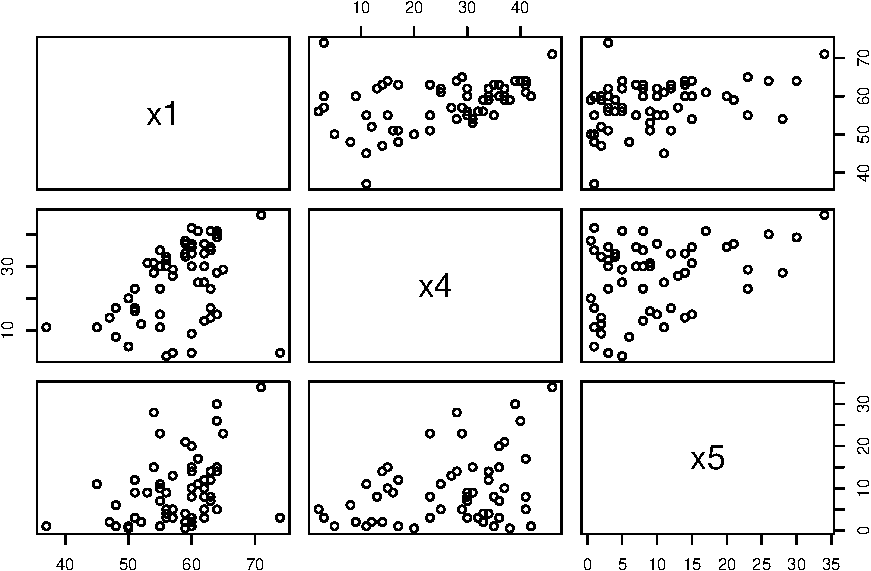
\includegraphics[keepaspectratio]{report_files/report_files/figure-latex/unnamed-chunk-2-1.pdf}}

\begin{Shaded}
\begin{Highlighting}[]
\CommentTok{\#iii)}
\NormalTok{agemodel }\OtherTok{\textless{}{-}} \FunctionTok{lm}\NormalTok{(x1}\SpecialCharTok{\textasciitilde{}}\NormalTok{x2}\SpecialCharTok{+}\NormalTok{x4}\SpecialCharTok{+}\NormalTok{x5}\SpecialCharTok{+}\NormalTok{x6}\SpecialCharTok{+}\NormalTok{x7}\SpecialCharTok{+}\NormalTok{x8}\SpecialCharTok{+}\NormalTok{x9)}
\FunctionTok{summary}\NormalTok{(agemodel)}
\end{Highlighting}
\end{Shaded}

\begin{verbatim}
## 
## Call:
## lm(formula = x1 ~ x2 + x4 + x5 + x6 + x7 + x8 + x9)
## 
## Residuals:
##      Min       1Q   Median       3Q      Max 
## -14.0663  -2.7035   0.0506   2.9182  19.2603 
## 
## Coefficients:
##               Estimate Std. Error t value Pr(>|t|)    
## (Intercept)  5.589e+01  3.090e+00  18.089   <2e-16 ***
## x2          -2.245e+00  1.404e+00  -1.599   0.1159    
## x4           1.743e-01  8.106e-02   2.150   0.0362 *  
## x5           2.137e-01  1.148e-01   1.861   0.0684 .  
## x6          -6.308e-05  1.847e-04  -0.341   0.7341    
## x7           7.964e-03  7.326e-03   1.087   0.2820    
## x8          -6.128e-01  3.196e-01  -1.918   0.0607 .  
## x9          -2.355e-04  3.848e-03  -0.061   0.9514    
## ---
## Signif. codes:  0 '***' 0.001 '**' 0.01 '*' 0.05 '.' 0.1 ' ' 1
## 
## Residual standard error: 5.588 on 52 degrees of freedom
## Multiple R-squared:  0.2956, Adjusted R-squared:  0.2008 
## F-statistic: 3.118 on 7 and 52 DF,  p-value: 0.007999
\end{verbatim}

\begin{Shaded}
\begin{Highlighting}[]
\NormalTok{VIF }\OtherTok{\textless{}{-}} \DecValTok{1}\SpecialCharTok{/}\NormalTok{(}\DecValTok{1}\FloatTok{{-}0.2956}\NormalTok{)}
\CommentTok{\#its ok}
\CommentTok{\#e)}
\NormalTok{new\_x }\OtherTok{\textless{}{-}} \FunctionTok{data.frame}\NormalTok{(}\AttributeTok{x1=}\DecValTok{48}\NormalTok{,}\AttributeTok{x2=}\DecValTok{1}\NormalTok{,}\AttributeTok{x4=}\DecValTok{14}\NormalTok{,}\AttributeTok{x5=}\DecValTok{3}\NormalTok{,}\AttributeTok{x6=}\DecValTok{3100}\NormalTok{,}\AttributeTok{x7=}\FloatTok{2.1}\NormalTok{,}\AttributeTok{x8=}\FloatTok{1.1}\NormalTok{,}\AttributeTok{x9=}\DecValTok{172}\NormalTok{)}
\FunctionTok{predict}\NormalTok{(redmodel,new\_x,}\AttributeTok{interval=}\StringTok{\textquotesingle{}prediction\textquotesingle{}}\NormalTok{,}\AttributeTok{level=}\NormalTok{.}\DecValTok{95}\NormalTok{)}
\end{Highlighting}
\end{Shaded}

\begin{verbatim}
##        fit       lwr      upr
## 1 761.5257 -268.8854 1791.937
\end{verbatim}

\section{FROM HERE ON IS THE START OF
A3}\label{from-here-on-is-the-start-of-a3}

\section{Question 1}\label{question-1}

The residual vs fitted plot is fairly regular, nothing too out of the
blue. Some outliers, but that's to be expected.

\begin{Shaded}
\begin{Highlighting}[]
\FunctionTok{plot}\NormalTok{(redmodel, }\AttributeTok{which =} \DecValTok{1}\NormalTok{)}
\end{Highlighting}
\end{Shaded}

\pandocbounded{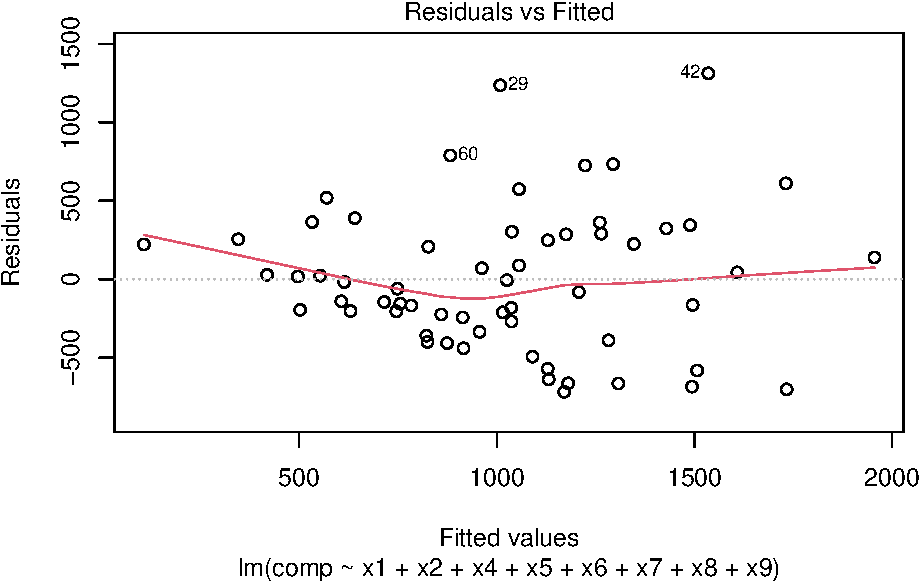
\includegraphics[keepaspectratio]{report_files/report_files/figure-latex/unnamed-chunk-3-1.pdf}}

The QQ is also rather normal, hinting at a slight right skew, but
overall I think it's meets expectations of being roughly normally
distributed.

\begin{Shaded}
\begin{Highlighting}[]
\FunctionTok{plot}\NormalTok{(redmodel, }\AttributeTok{which =} \DecValTok{2}\NormalTok{)}
\end{Highlighting}
\end{Shaded}

\pandocbounded{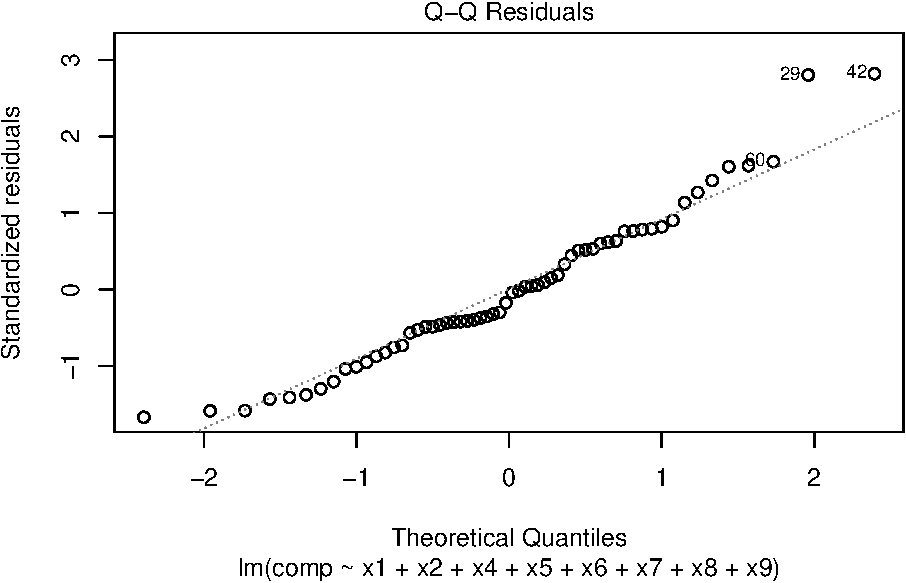
\includegraphics[keepaspectratio]{report_files/report_files/figure-latex/unnamed-chunk-4-1.pdf}}

\section{Question 2}\label{question-2}

\subsubsection{a)}\label{a}

\begin{Shaded}
\begin{Highlighting}[]
\FunctionTok{hist}\NormalTok{(comp)}
\end{Highlighting}
\end{Shaded}

\pandocbounded{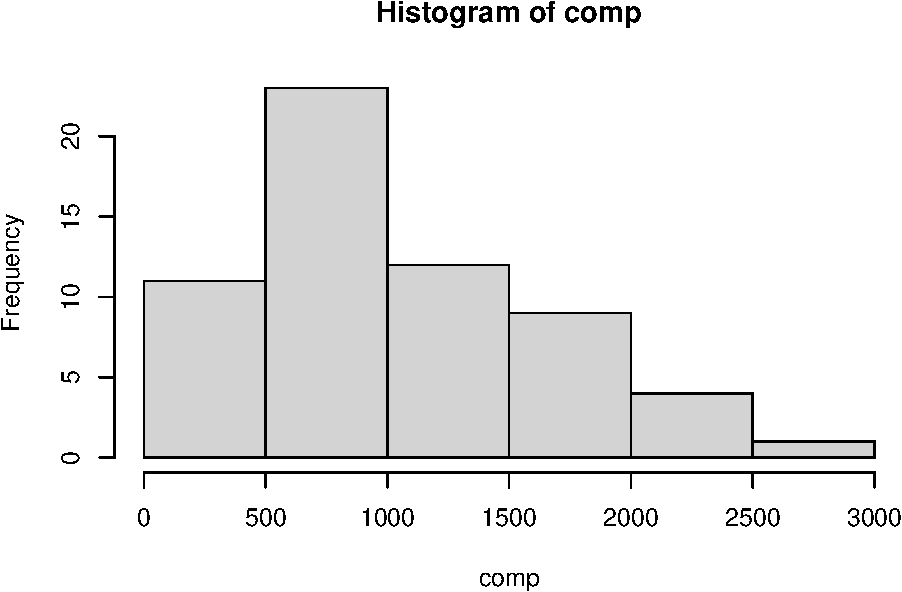
\includegraphics[keepaspectratio]{report_files/report_files/figure-latex/unnamed-chunk-5-1.pdf}}

it has a heavy right tail, so using ln as a transform would send the
outliers a lot closer to the rest of the data.

\subsubsection{b)}\label{b}

\begin{Shaded}
\begin{Highlighting}[]
\NormalTok{lncomp }\OtherTok{\textless{}{-}} \FunctionTok{log}\NormalTok{(comp)}
\NormalTok{lnredmodel }\OtherTok{\textless{}{-}} \FunctionTok{lm}\NormalTok{(lncomp }\SpecialCharTok{\textasciitilde{}}\NormalTok{ x1}\SpecialCharTok{+}\NormalTok{x2}\SpecialCharTok{+}\NormalTok{x4}\SpecialCharTok{+}\NormalTok{x5}\SpecialCharTok{+}\NormalTok{x6}\SpecialCharTok{+}\NormalTok{x7}\SpecialCharTok{+}\NormalTok{x8}\SpecialCharTok{+}\NormalTok{x9)}
\end{Highlighting}
\end{Shaded}

\subsubsection{c)}\label{c}

\begin{Shaded}
\begin{Highlighting}[]
\FunctionTok{summary}\NormalTok{(lnredmodel)}
\end{Highlighting}
\end{Shaded}

\begin{verbatim}
## 
## Call:
## lm(formula = lncomp ~ x1 + x2 + x4 + x5 + x6 + x7 + x8 + x9)
## 
## Residuals:
##      Min       1Q   Median       3Q      Max 
## -0.78408 -0.28263 -0.03879  0.33245  0.91600 
## 
## Coefficients:
##               Estimate Std. Error t value Pr(>|t|)    
## (Intercept)  6.056e+00  6.680e-01   9.066 3.27e-12 ***
## x1           8.821e-03  1.110e-02   0.795   0.4305    
## x2          -2.093e-01  1.151e-01  -1.818   0.0750 .  
## x4           1.066e-02  6.771e-03   1.574   0.1218    
## x5           1.384e-02  9.493e-03   1.458   0.1509    
## x6           1.744e-05  1.481e-05   1.178   0.2442    
## x7           1.013e-03  5.931e-04   1.708   0.0936 .  
## x8          -6.259e-02  2.647e-02  -2.364   0.0219 *  
## x9           4.131e-04  3.081e-04   1.341   0.1859    
## ---
## Signif. codes:  0 '***' 0.001 '**' 0.01 '*' 0.05 '.' 0.1 ' ' 1
## 
## Residual standard error: 0.4473 on 51 degrees of freedom
## Multiple R-squared:  0.4391, Adjusted R-squared:  0.3511 
## F-statistic: 4.991 on 8 and 51 DF,  p-value: 0.000134
\end{verbatim}

\begin{Shaded}
\begin{Highlighting}[]
\FunctionTok{summary}\NormalTok{(redmodel)}
\end{Highlighting}
\end{Shaded}

\begin{verbatim}
## 
## Call:
## lm(formula = comp ~ x1 + x2 + x4 + x5 + x6 + x7 + x8 + x9)
## 
## Residuals:
##     Min      1Q  Median      3Q     Max 
## -717.60 -285.72  -39.28  286.79 1311.98 
## 
## Coefficients:
##               Estimate Std. Error t value Pr(>|t|)  
## (Intercept)  277.33972  730.43905   0.380   0.7058  
## x1             9.17031   12.13919   0.755   0.4535  
## x2          -212.08401  125.88116  -1.685   0.0981 .
## x4            10.44381    7.40399   1.411   0.1644  
## x5            15.04509   10.37970   1.449   0.1533  
## x6             0.01059    0.01619   0.654   0.5158  
## x7             0.88585    0.64852   1.366   0.1779  
## x8           -59.34763   28.94672  -2.050   0.0455 *
## x9             0.55425    0.33688   1.645   0.1061  
## ---
## Signif. codes:  0 '***' 0.001 '**' 0.01 '*' 0.05 '.' 0.1 ' ' 1
## 
## Residual standard error: 489.1 on 51 degrees of freedom
## Multiple R-squared:  0.4042, Adjusted R-squared:  0.3108 
## F-statistic: 4.325 on 8 and 51 DF,  p-value: 0.0004988
\end{verbatim}

we see a very slight improvement in the model in which we applied log to
the compensation.

\subsubsection{d)}\label{d}

\begin{Shaded}
\begin{Highlighting}[]
\FunctionTok{plot}\NormalTok{(lnredmodel, }\AttributeTok{which =} \DecValTok{1}\NormalTok{)}
\end{Highlighting}
\end{Shaded}

\pandocbounded{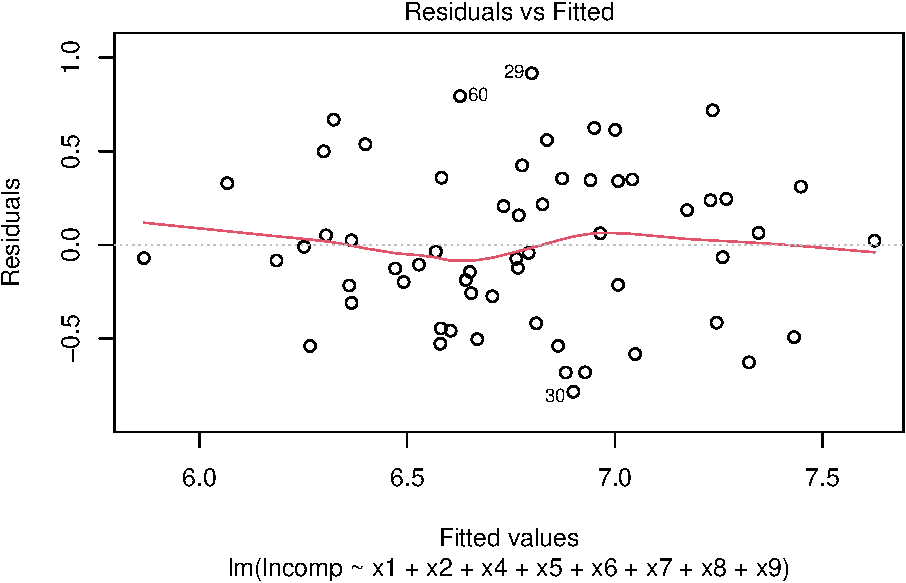
\includegraphics[keepaspectratio]{report_files/report_files/figure-latex/unnamed-chunk-8-1.pdf}}

I personally don't see a substantial difference in the res vs the
fitted, but that's about normal for my human eyes.

\begin{Shaded}
\begin{Highlighting}[]
\FunctionTok{plot}\NormalTok{(lnredmodel, }\AttributeTok{which =} \DecValTok{2}\NormalTok{)}
\end{Highlighting}
\end{Shaded}

\pandocbounded{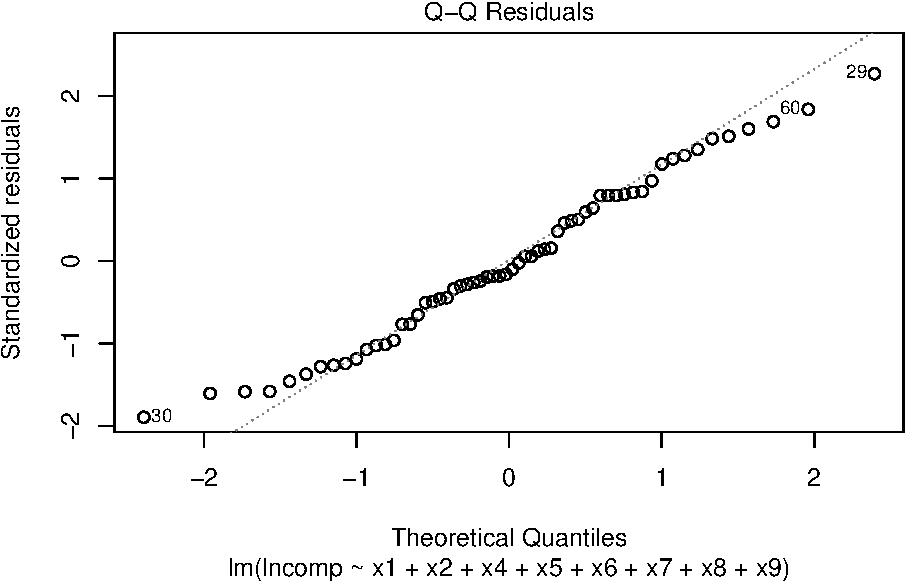
\includegraphics[keepaspectratio]{report_files/report_files/figure-latex/unnamed-chunk-9-1.pdf}}

Here I notice that the skew is gone from before, but there is slightly
lighter tails than expected of a normal distribution.

\section{Question 3}\label{question-3}

\subsubsection{a)}\label{a-1}

\begin{Shaded}
\begin{Highlighting}[]
\FunctionTok{plot}\NormalTok{(x6,lncomp)}
\end{Highlighting}
\end{Shaded}

\pandocbounded{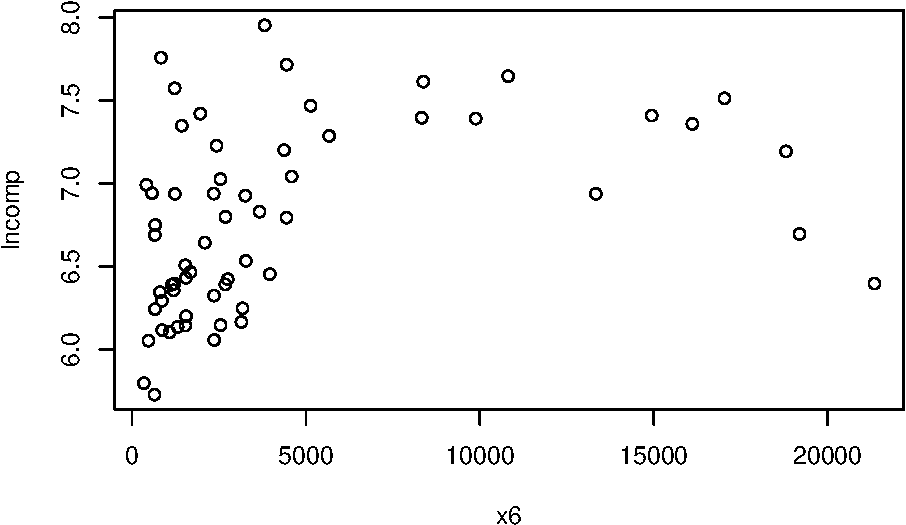
\includegraphics[keepaspectratio]{report_files/report_files/figure-latex/unnamed-chunk-10-1.pdf}}

Given the sales and log of compensation, it doesn't really seem like a
linear model would be a good fit, the data doesn't seem to have a strong
linear relation.

\subsubsection{b)}\label{b-1}

\begin{Shaded}
\begin{Highlighting}[]
\FunctionTok{plot}\NormalTok{(}\FunctionTok{log}\NormalTok{(x6),lncomp)}
\end{Highlighting}
\end{Shaded}

\pandocbounded{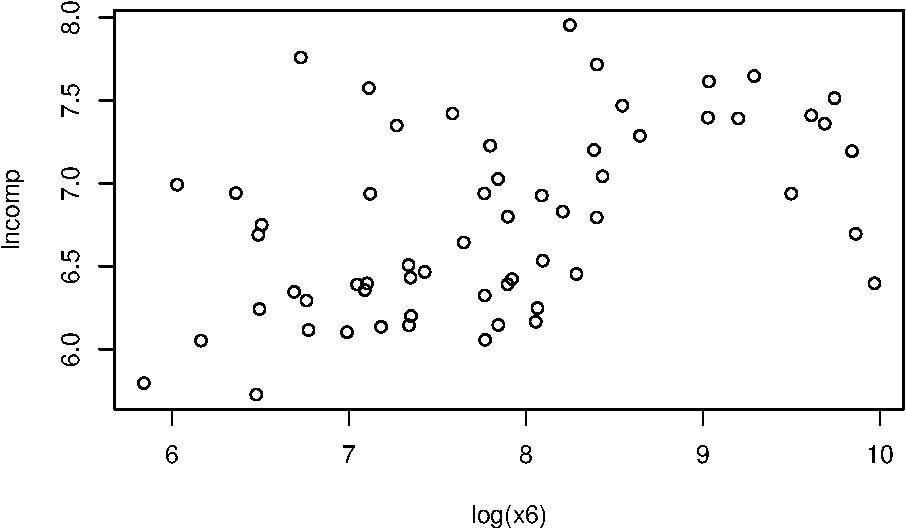
\includegraphics[keepaspectratio]{report_files/report_files/figure-latex/unnamed-chunk-11-1.pdf}}

We see a slightly better linear relation, but it's still not
particularly clear, especially on the far right side.

\subsubsection{c)}\label{c-1}

\begin{Shaded}
\begin{Highlighting}[]
\NormalTok{lnmodel }\OtherTok{\textless{}{-}} \FunctionTok{lm}\NormalTok{(lncomp }\SpecialCharTok{\textasciitilde{}} \FunctionTok{log}\NormalTok{(x6)}\SpecialCharTok{+}\FunctionTok{log}\NormalTok{(x7)}\SpecialCharTok{+}\FunctionTok{log}\NormalTok{(x8)}\SpecialCharTok{+}\FunctionTok{log}\NormalTok{(x9))}
\FunctionTok{summary}\NormalTok{(lnmodel)  }
\end{Highlighting}
\end{Shaded}

\begin{verbatim}
## 
## Call:
## lm(formula = lncomp ~ log(x6) + log(x7) + log(x8) + log(x9))
## 
## Residuals:
##      Min       1Q   Median       3Q      Max 
## -0.77458 -0.33331 -0.07043  0.29030  1.19390 
## 
## Coefficients:
##             Estimate Std. Error t value Pr(>|t|)    
## (Intercept)  5.49990    0.51439  10.692 4.81e-15 ***
## log(x6)      0.09903    0.08656   1.144  0.25755    
## log(x7)      0.29297    0.10152   2.886  0.00557 ** 
## log(x8)     -0.24594    0.10592  -2.322  0.02397 *  
## log(x9)     -0.06740    0.10216  -0.660  0.51217    
## ---
## Signif. codes:  0 '***' 0.001 '**' 0.01 '*' 0.05 '.' 0.1 ' ' 1
## 
## Residual standard error: 0.4585 on 55 degrees of freedom
## Multiple R-squared:  0.3644, Adjusted R-squared:  0.3182 
## F-statistic: 7.884 on 4 and 55 DF,  p-value: 4.261e-05
\end{verbatim}

We can notice that the log of x7(Val), and log of x8(PCTOWN) have p
values of significance, so we expect that these would explain more of
the variation than the other 2 variates. Overall, it is a weaker model,
with a smaller adj R\^{}2 than the model previously, which only took the
log of the response variate.

\section{Question 4}\label{question-4}

\begin{Shaded}
\begin{Highlighting}[]
\FunctionTok{plot}\NormalTok{(lnmodel, }\AttributeTok{which =} \DecValTok{1}\NormalTok{)}
\end{Highlighting}
\end{Shaded}

\pandocbounded{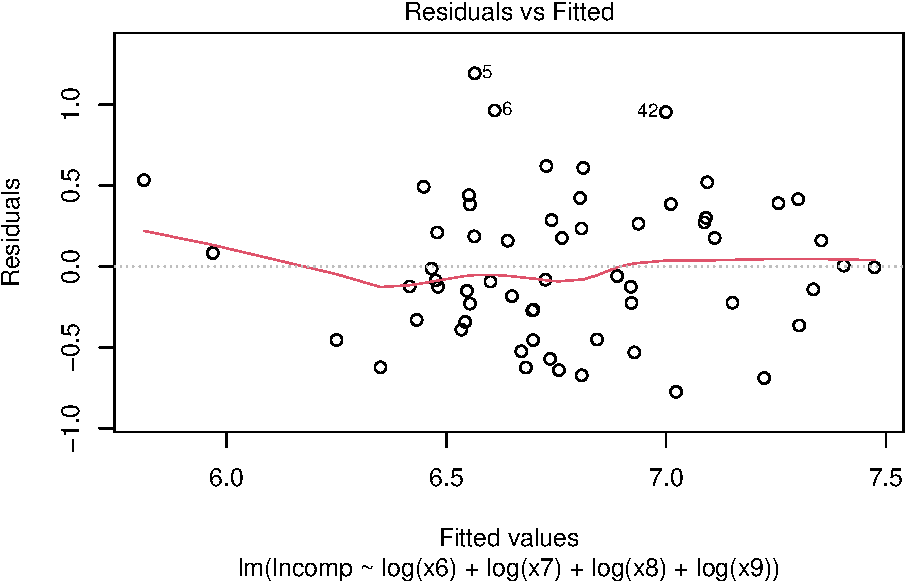
\includegraphics[keepaspectratio]{report_files/report_files/figure-latex/unnamed-chunk-13-1.pdf}}

It is getting marginally better, with a flatter line, concentrating at
0.

\begin{Shaded}
\begin{Highlighting}[]
\FunctionTok{plot}\NormalTok{(lnmodel, }\AttributeTok{which =} \DecValTok{2}\NormalTok{)}
\end{Highlighting}
\end{Shaded}

\pandocbounded{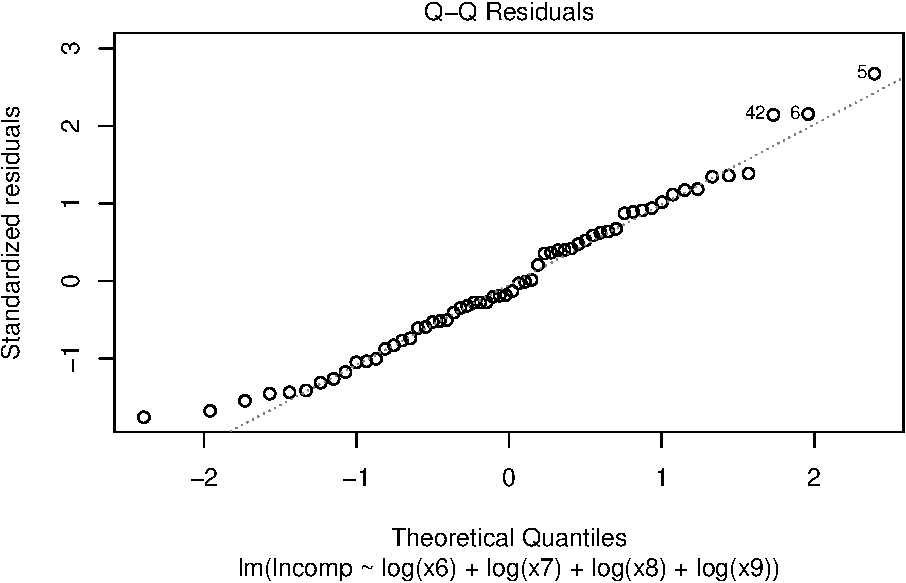
\includegraphics[keepaspectratio]{report_files/report_files/figure-latex/unnamed-chunk-14-1.pdf}}
The tails now are not as light as previous, so that's a bit more
adequate.

\section{Question 5}\label{question-5}

\begin{Shaded}
\begin{Highlighting}[]
\FunctionTok{plot}\NormalTok{(}\FunctionTok{fitted}\NormalTok{(lnmodel),}\FunctionTok{rstudent}\NormalTok{(lnmodel))}
\FunctionTok{abline}\NormalTok{(}\AttributeTok{h=}\DecValTok{0}\NormalTok{)}
\end{Highlighting}
\end{Shaded}

\pandocbounded{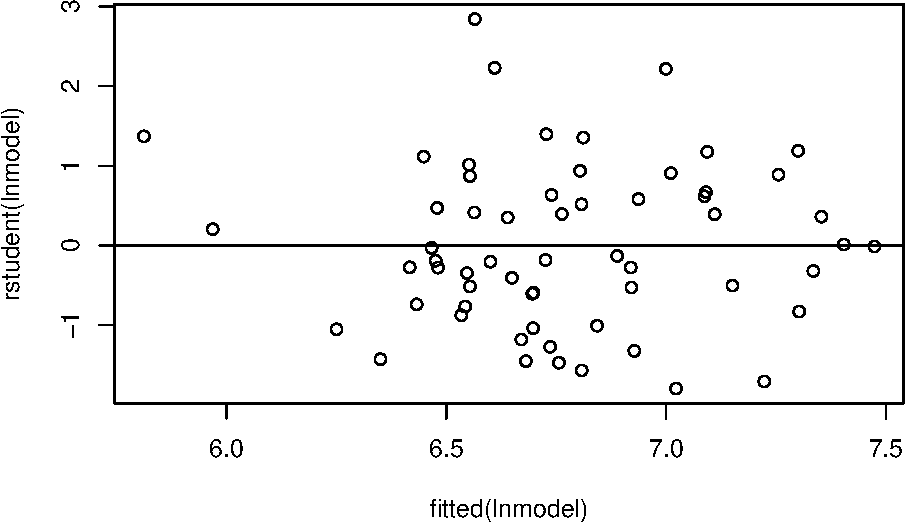
\includegraphics[keepaspectratio]{report_files/report_files/figure-latex/unnamed-chunk-15-1.pdf}}

We see that it is really similar to the previous plot.

\begin{Shaded}
\begin{Highlighting}[]
\FunctionTok{qqnorm}\NormalTok{(}\FunctionTok{rstudent}\NormalTok{(lnmodel)); }\FunctionTok{qqline}\NormalTok{(}\FunctionTok{rstudent}\NormalTok{(lnmodel))}
\end{Highlighting}
\end{Shaded}

\pandocbounded{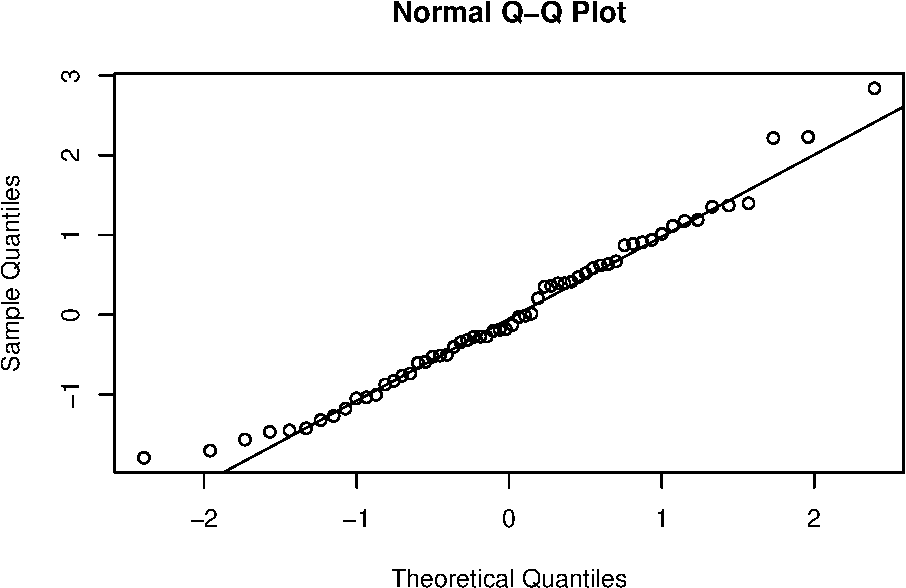
\includegraphics[keepaspectratio]{report_files/report_files/figure-latex/unnamed-chunk-16-1.pdf}}
Same here, it is rather similar.

\section{Question 6}\label{question-6}

remember that p = 4, n = 60, so we consider `high-leverage' to be:

\begin{Shaded}
\begin{Highlighting}[]
\NormalTok{highlev }\OtherTok{=} \DecValTok{2}\SpecialCharTok{*}\NormalTok{(}\DecValTok{4}\SpecialCharTok{+}\DecValTok{1}\NormalTok{)}\SpecialCharTok{/}\DecValTok{60}
\NormalTok{highlev}
\end{Highlighting}
\end{Shaded}

\begin{verbatim}
## [1] 0.1666667
\end{verbatim}

\begin{Shaded}
\begin{Highlighting}[]
\FunctionTok{plot}\NormalTok{(}\FunctionTok{hatvalues}\NormalTok{(lnmodel))}
\FunctionTok{abline}\NormalTok{(}\AttributeTok{h =}\NormalTok{ highlev)}
\end{Highlighting}
\end{Shaded}

\pandocbounded{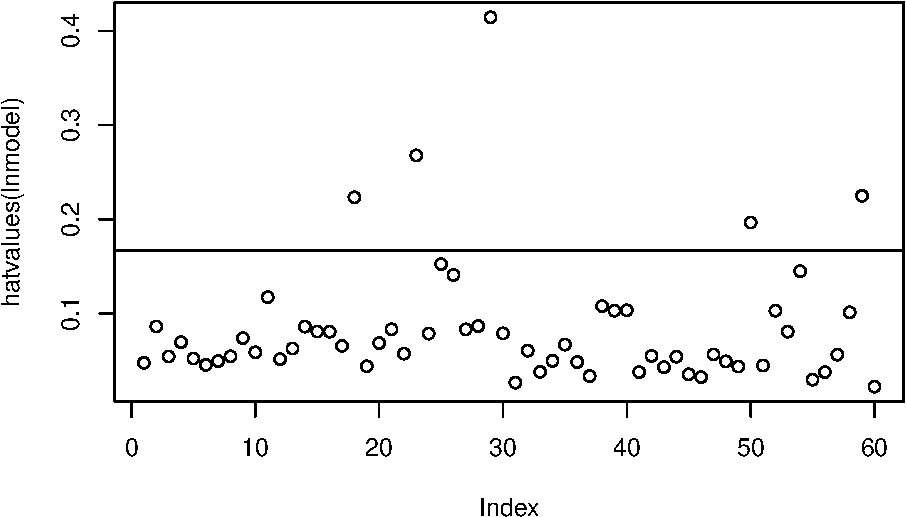
\includegraphics[keepaspectratio]{report_files/report_files/figure-latex/unnamed-chunk-18-1.pdf}}
We see there is indeed a big outlier. Let's investigate.

\section{Question 7}\label{question-7}

Here is the highest leverage index:

\begin{Shaded}
\begin{Highlighting}[]
\FunctionTok{which.max}\NormalTok{(}\FunctionTok{hatvalues}\NormalTok{(lnmodel))}
\end{Highlighting}
\end{Shaded}

\begin{verbatim}
## 29 
## 29
\end{verbatim}

Here are the plots of the explanatory variates with the 29th index
highlighted:

\begin{Shaded}
\begin{Highlighting}[]
\FunctionTok{plot}\NormalTok{(}\FunctionTok{log}\NormalTok{(x6))}
\FunctionTok{points}\NormalTok{(}\DecValTok{29}\NormalTok{,}\FunctionTok{log}\NormalTok{(x6)[}\DecValTok{29}\NormalTok{], }\AttributeTok{col =} \StringTok{"red"}\NormalTok{, }\AttributeTok{pch =} \DecValTok{16}\NormalTok{, }\AttributeTok{cex =} \FloatTok{2.5}\NormalTok{)}
\end{Highlighting}
\end{Shaded}

\pandocbounded{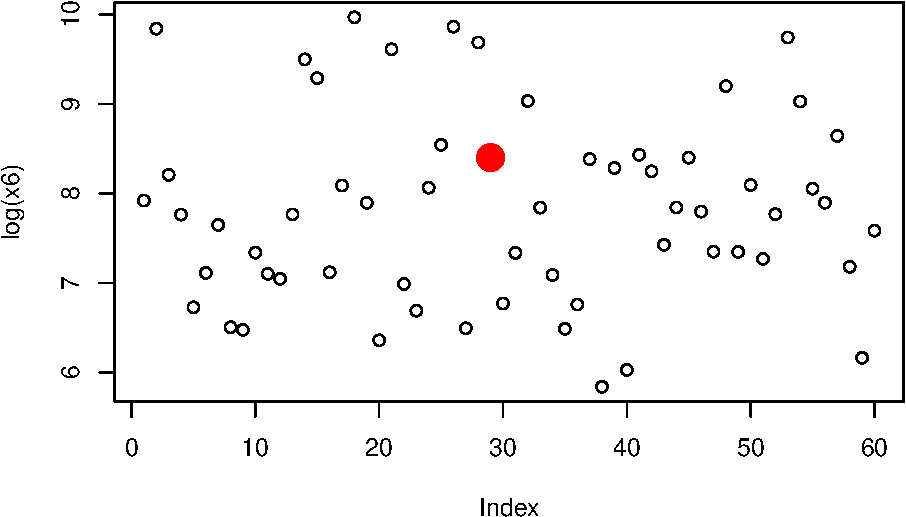
\includegraphics[keepaspectratio]{report_files/report_files/figure-latex/unnamed-chunk-20-1.pdf}}

\begin{Shaded}
\begin{Highlighting}[]
\FunctionTok{plot}\NormalTok{(}\FunctionTok{log}\NormalTok{(x7))}
\FunctionTok{points}\NormalTok{(}\DecValTok{29}\NormalTok{,}\FunctionTok{log}\NormalTok{(x7)[}\DecValTok{29}\NormalTok{], }\AttributeTok{col =} \StringTok{"red"}\NormalTok{, }\AttributeTok{pch =} \DecValTok{16}\NormalTok{, }\AttributeTok{cex =} \FloatTok{2.5}\NormalTok{)}
\end{Highlighting}
\end{Shaded}

\pandocbounded{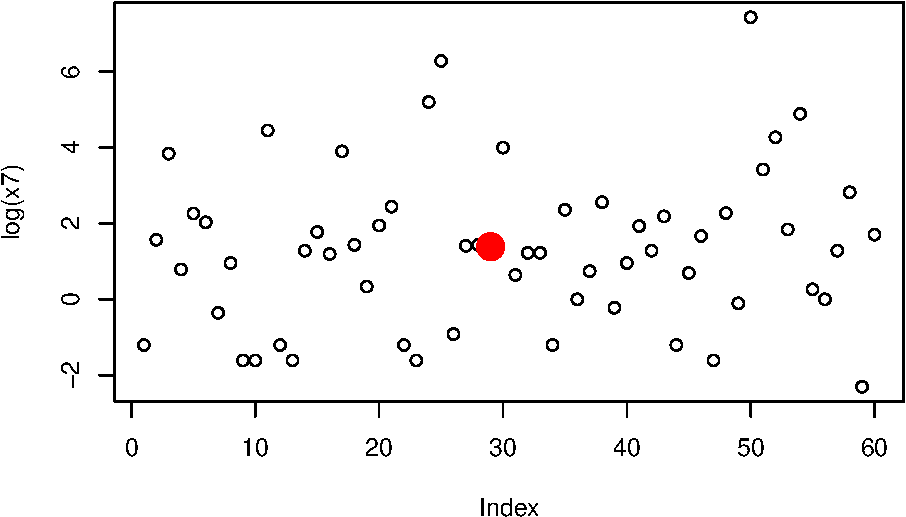
\includegraphics[keepaspectratio]{report_files/report_files/figure-latex/unnamed-chunk-21-1.pdf}}

\begin{Shaded}
\begin{Highlighting}[]
\FunctionTok{plot}\NormalTok{(}\FunctionTok{log}\NormalTok{(x8))}
\FunctionTok{points}\NormalTok{(}\DecValTok{29}\NormalTok{,}\FunctionTok{log}\NormalTok{(x8)[}\DecValTok{29}\NormalTok{], }\AttributeTok{col =} \StringTok{"red"}\NormalTok{, }\AttributeTok{pch =} \DecValTok{16}\NormalTok{, }\AttributeTok{cex =} \FloatTok{2.5}\NormalTok{)}
\end{Highlighting}
\end{Shaded}

\pandocbounded{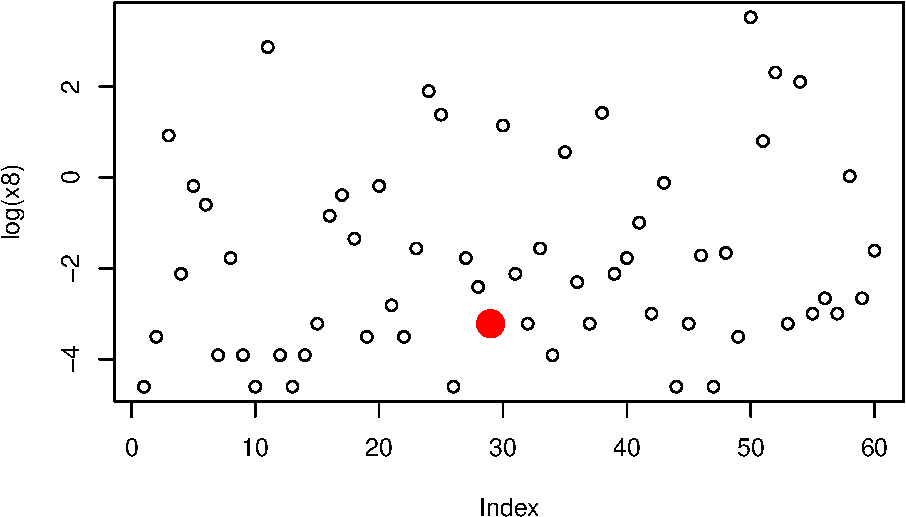
\includegraphics[keepaspectratio]{report_files/report_files/figure-latex/unnamed-chunk-22-1.pdf}}

\begin{Shaded}
\begin{Highlighting}[]
\FunctionTok{plot}\NormalTok{(}\FunctionTok{log}\NormalTok{(x9))}
\FunctionTok{points}\NormalTok{(}\DecValTok{29}\NormalTok{,}\FunctionTok{log}\NormalTok{(x9)[}\DecValTok{29}\NormalTok{], }\AttributeTok{col =} \StringTok{"red"}\NormalTok{, }\AttributeTok{pch =} \DecValTok{16}\NormalTok{, }\AttributeTok{cex =} \FloatTok{2.5}\NormalTok{)}
\end{Highlighting}
\end{Shaded}

\pandocbounded{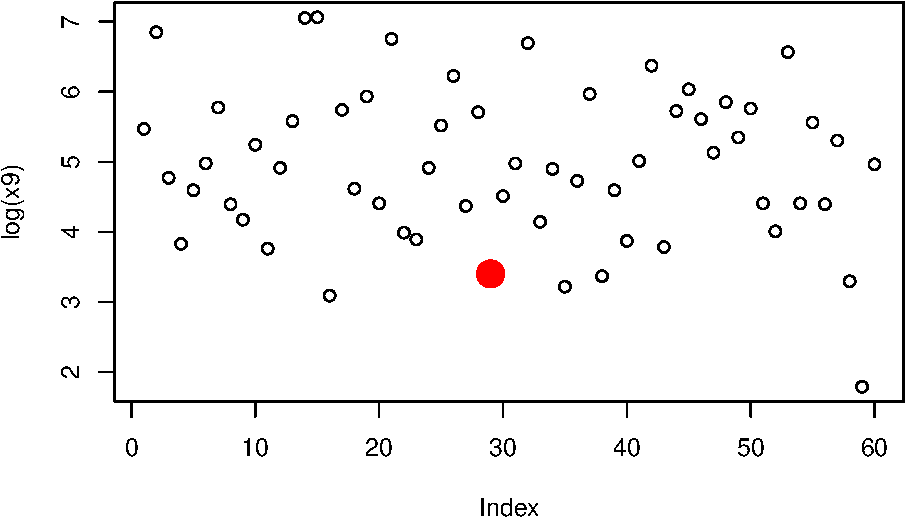
\includegraphics[keepaspectratio]{report_files/report_files/figure-latex/unnamed-chunk-23-1.pdf}}

I'd say that only in the log(x9), log of the profit, do we see index 29
being particularly outlier-ish.

\section{Question 8}\label{question-8}

\begin{Shaded}
\begin{Highlighting}[]
\FunctionTok{plot}\NormalTok{(lnmodel, }\AttributeTok{which =} \DecValTok{4}\NormalTok{)}
\end{Highlighting}
\end{Shaded}

\pandocbounded{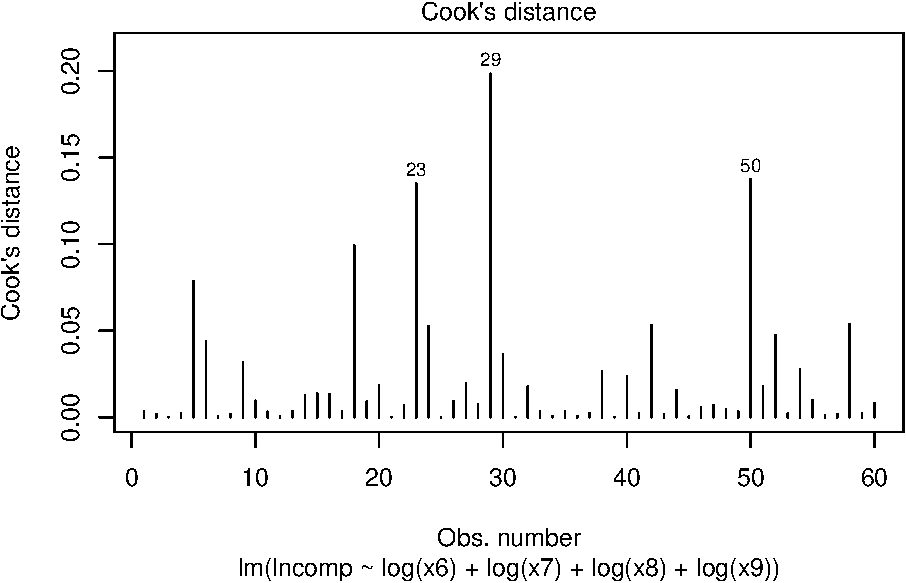
\includegraphics[keepaspectratio]{report_files/report_files/figure-latex/unnamed-chunk-24-1.pdf}}

We see that the 29th index is indeed the most influential, but according
to our general rule in class, it isn't greater than 1, so we don't
conclude it has `high' influence, even though comparatively it has the
highest influence.

\section{Question 9}\label{question-9}

\subsubsection{a)}\label{a-2}

let's start with the full model from question 3:

\begin{Shaded}
\begin{Highlighting}[]
\FunctionTok{summary}\NormalTok{(lnmodel)}
\end{Highlighting}
\end{Shaded}

\begin{verbatim}
## 
## Call:
## lm(formula = lncomp ~ log(x6) + log(x7) + log(x8) + log(x9))
## 
## Residuals:
##      Min       1Q   Median       3Q      Max 
## -0.77458 -0.33331 -0.07043  0.29030  1.19390 
## 
## Coefficients:
##             Estimate Std. Error t value Pr(>|t|)    
## (Intercept)  5.49990    0.51439  10.692 4.81e-15 ***
## log(x6)      0.09903    0.08656   1.144  0.25755    
## log(x7)      0.29297    0.10152   2.886  0.00557 ** 
## log(x8)     -0.24594    0.10592  -2.322  0.02397 *  
## log(x9)     -0.06740    0.10216  -0.660  0.51217    
## ---
## Signif. codes:  0 '***' 0.001 '**' 0.01 '*' 0.05 '.' 0.1 ' ' 1
## 
## Residual standard error: 0.4585 on 55 degrees of freedom
## Multiple R-squared:  0.3644, Adjusted R-squared:  0.3182 
## F-statistic: 7.884 on 4 and 55 DF,  p-value: 4.261e-05
\end{verbatim}

Since log(x9) has the highest p value that is also above 0.15, we drop
it:

\begin{Shaded}
\begin{Highlighting}[]
\NormalTok{droppedx9 }\OtherTok{\textless{}{-}} \FunctionTok{lm}\NormalTok{(lncomp }\SpecialCharTok{\textasciitilde{}} \FunctionTok{log}\NormalTok{(x6)}\SpecialCharTok{+}\FunctionTok{log}\NormalTok{(x7)}\SpecialCharTok{+}\FunctionTok{log}\NormalTok{(x8))}
\FunctionTok{summary}\NormalTok{(droppedx9)}
\end{Highlighting}
\end{Shaded}

\begin{verbatim}
## 
## Call:
## lm(formula = lncomp ~ log(x6) + log(x7) + log(x8))
## 
## Residuals:
##      Min       1Q   Median       3Q      Max 
## -0.78287 -0.31337 -0.08203  0.30202  1.16428 
## 
## Coefficients:
##             Estimate Std. Error t value Pr(>|t|)    
## (Intercept)  5.42552    0.49934  10.865 2.07e-15 ***
## log(x6)      0.08310    0.08270   1.005  0.31931    
## log(x7)      0.25316    0.08123   3.117  0.00289 ** 
## log(x8)     -0.20022    0.07971  -2.512  0.01491 *  
## ---
## Signif. codes:  0 '***' 0.001 '**' 0.01 '*' 0.05 '.' 0.1 ' ' 1
## 
## Residual standard error: 0.4562 on 56 degrees of freedom
## Multiple R-squared:  0.3594, Adjusted R-squared:  0.3251 
## F-statistic: 10.47 on 3 and 56 DF,  p-value: 1.436e-05
\end{verbatim}

Since log(x6) has the highest p value above 0.15, we drop it:

\begin{Shaded}
\begin{Highlighting}[]
\NormalTok{droppedx9x6 }\OtherTok{\textless{}{-}} \FunctionTok{lm}\NormalTok{(lncomp }\SpecialCharTok{\textasciitilde{}} \FunctionTok{log}\NormalTok{(x7)}\SpecialCharTok{+}\FunctionTok{log}\NormalTok{(x8))}
\FunctionTok{summary}\NormalTok{(droppedx9x6)}
\end{Highlighting}
\end{Shaded}

\begin{verbatim}
## 
## Call:
## lm(formula = lncomp ~ log(x7) + log(x8))
## 
## Residuals:
##      Min       1Q   Median       3Q      Max 
## -0.77616 -0.32415 -0.06035  0.35129  1.11142 
## 
## Coefficients:
##             Estimate Std. Error t value Pr(>|t|)    
## (Intercept)  5.89419    0.17832  33.053  < 2e-16 ***
## log(x7)      0.31175    0.05656   5.512 8.94e-07 ***
## log(x8)     -0.25792    0.05528  -4.665 1.91e-05 ***
## ---
## Signif. codes:  0 '***' 0.001 '**' 0.01 '*' 0.05 '.' 0.1 ' ' 1
## 
## Residual standard error: 0.4563 on 57 degrees of freedom
## Multiple R-squared:  0.3478, Adjusted R-squared:  0.325 
## F-statistic:  15.2 on 2 and 57 DF,  p-value: 5.119e-06
\end{verbatim}

Since no other explanatory variate is above 0.15, we keep this as our
model.

\subsubsection{b)}\label{b-2}

\begin{Shaded}
\begin{Highlighting}[]
\NormalTok{lnX }\OtherTok{\textless{}{-}} \FunctionTok{as.matrix}\NormalTok{(}\FunctionTok{cbind}\NormalTok{(}\FunctionTok{log}\NormalTok{(x6),}\FunctionTok{log}\NormalTok{(x7),}\FunctionTok{log}\NormalTok{(x8),}\FunctionTok{log}\NormalTok{(x9)))}
\NormalTok{cp\_out    }\OtherTok{\textless{}{-}} \FunctionTok{leaps}\NormalTok{(}\AttributeTok{x =}\NormalTok{ lnX, }\AttributeTok{y =}\NormalTok{ lncomp, }\AttributeTok{method =} \StringTok{"Cp"}\NormalTok{,    }\AttributeTok{nbest =} \DecValTok{1}\NormalTok{)}
\NormalTok{adjr2\_out }\OtherTok{\textless{}{-}} \FunctionTok{leaps}\NormalTok{(}\AttributeTok{x =}\NormalTok{ lnX, }\AttributeTok{y =}\NormalTok{ lncomp, }\AttributeTok{method =} \StringTok{"adjr2"}\NormalTok{, }\AttributeTok{nbest =} \DecValTok{1}\NormalTok{)}
\NormalTok{cp\_out}\SpecialCharTok{$}\NormalTok{Cp    }
\end{Highlighting}
\end{Shaded}

\begin{verbatim}
## [1] 10.237745  2.434732  3.435257  5.000000
\end{verbatim}

\begin{Shaded}
\begin{Highlighting}[]
\NormalTok{cp\_out}\SpecialCharTok{$}\NormalTok{which  }
\end{Highlighting}
\end{Shaded}

\begin{verbatim}
##       1     2     3     4
## 1  TRUE FALSE FALSE FALSE
## 2 FALSE  TRUE  TRUE FALSE
## 3  TRUE  TRUE  TRUE FALSE
## 4  TRUE  TRUE  TRUE  TRUE
\end{verbatim}

\begin{Shaded}
\begin{Highlighting}[]
\NormalTok{adjr2\_out}\SpecialCharTok{$}\NormalTok{adjr2 }
\end{Highlighting}
\end{Shaded}

\begin{verbatim}
## [1] 0.2213539 0.3249527 0.3250671 0.3181912
\end{verbatim}

We pick log(x6), log(x7) and log(x8), bc its the highest
adjR\^{}2(barely though) that fits our mallows cp of being strictly less
than k+1.

\begin{Shaded}
\begin{Highlighting}[]
\NormalTok{pickedmodel }\OtherTok{\textless{}{-}} \FunctionTok{lm}\NormalTok{(lncomp }\SpecialCharTok{\textasciitilde{}} \FunctionTok{log}\NormalTok{(x6)}\SpecialCharTok{+}\FunctionTok{log}\NormalTok{(x7)}\SpecialCharTok{+}\FunctionTok{log}\NormalTok{(x8))}
\end{Highlighting}
\end{Shaded}

\subsubsection{c)}\label{c-2}

\begin{Shaded}
\begin{Highlighting}[]
\NormalTok{n }\OtherTok{\textless{}{-}} \FunctionTok{length}\NormalTok{(lncomp)}
\NormalTok{mse\_full }\OtherTok{\textless{}{-}} \FunctionTok{summary}\NormalTok{(lnmodel)}\SpecialCharTok{$}\NormalTok{sigma}\SpecialCharTok{\^{}}\DecValTok{2}   
\NormalTok{sse\_reduced }\OtherTok{\textless{}{-}} \FunctionTok{sum}\NormalTok{(}\FunctionTok{resid}\NormalTok{(pickedmodel)}\SpecialCharTok{\^{}}\DecValTok{2}\NormalTok{)  }
\NormalTok{k }\OtherTok{\textless{}{-}} \DecValTok{3}\SpecialCharTok{+}\DecValTok{1}                                

\NormalTok{Cp\_check }\OtherTok{\textless{}{-}}\NormalTok{ sse\_reduced}\SpecialCharTok{/}\NormalTok{mse\_full }\SpecialCharTok{{-}}\NormalTok{ (n }\SpecialCharTok{{-}} \DecValTok{2}\SpecialCharTok{*}\NormalTok{k)}
\NormalTok{Cp\_check}
\end{Highlighting}
\end{Shaded}

\begin{verbatim}
## [1] 3.435257
\end{verbatim}

Which is the same mallows cp as expected.

\subsubsection{d)}\label{d-1}

\begin{Shaded}
\begin{Highlighting}[]
\FunctionTok{summary}\NormalTok{(pickedmodel)}
\end{Highlighting}
\end{Shaded}

\begin{verbatim}
## 
## Call:
## lm(formula = lncomp ~ log(x6) + log(x7) + log(x8))
## 
## Residuals:
##      Min       1Q   Median       3Q      Max 
## -0.78287 -0.31337 -0.08203  0.30202  1.16428 
## 
## Coefficients:
##             Estimate Std. Error t value Pr(>|t|)    
## (Intercept)  5.42552    0.49934  10.865 2.07e-15 ***
## log(x6)      0.08310    0.08270   1.005  0.31931    
## log(x7)      0.25316    0.08123   3.117  0.00289 ** 
## log(x8)     -0.20022    0.07971  -2.512  0.01491 *  
## ---
## Signif. codes:  0 '***' 0.001 '**' 0.01 '*' 0.05 '.' 0.1 ' ' 1
## 
## Residual standard error: 0.4562 on 56 degrees of freedom
## Multiple R-squared:  0.3594, Adjusted R-squared:  0.3251 
## F-statistic: 10.47 on 3 and 56 DF,  p-value: 1.436e-05
\end{verbatim}

\begin{Shaded}
\begin{Highlighting}[]
\FunctionTok{summary}\NormalTok{(droppedx9x6)}
\end{Highlighting}
\end{Shaded}

\begin{verbatim}
## 
## Call:
## lm(formula = lncomp ~ log(x7) + log(x8))
## 
## Residuals:
##      Min       1Q   Median       3Q      Max 
## -0.77616 -0.32415 -0.06035  0.35129  1.11142 
## 
## Coefficients:
##             Estimate Std. Error t value Pr(>|t|)    
## (Intercept)  5.89419    0.17832  33.053  < 2e-16 ***
## log(x7)      0.31175    0.05656   5.512 8.94e-07 ***
## log(x8)     -0.25792    0.05528  -4.665 1.91e-05 ***
## ---
## Signif. codes:  0 '***' 0.001 '**' 0.01 '*' 0.05 '.' 0.1 ' ' 1
## 
## Residual standard error: 0.4563 on 57 degrees of freedom
## Multiple R-squared:  0.3478, Adjusted R-squared:  0.325 
## F-statistic:  15.2 on 2 and 57 DF,  p-value: 5.119e-06
\end{verbatim}

they are slightly different, but honestly its the exact same comparision
made with the leaps function, with both models fitting our mallows cp
criteria. Our picked model has 0.0001 more adj R\^{}2 value, which is
basically a negligible difference in my opinion.

\subsubsection{e)}\label{e}

\begin{Shaded}
\begin{Highlighting}[]
\FunctionTok{anova}\NormalTok{(pickedmodel,lnmodel)}
\end{Highlighting}
\end{Shaded}

\begin{verbatim}
## Analysis of Variance Table
## 
## Model 1: lncomp ~ log(x6) + log(x7) + log(x8)
## Model 2: lncomp ~ log(x6) + log(x7) + log(x8) + log(x9)
##   Res.Df    RSS Df Sum of Sq      F Pr(>F)
## 1     56 11.656                           
## 2     55 11.564  1  0.091517 0.4353 0.5122
\end{verbatim}

From the test, we cant really say with confidence the dropped log(x9)
variate, the log of the profit of the company, contributed significantly
to the log of the CEO compensation.

\subsubsection{f)}\label{f}

\begin{Shaded}
\begin{Highlighting}[]
\FunctionTok{plot}\NormalTok{(}\FunctionTok{fitted}\NormalTok{(pickedmodel), }\FunctionTok{rstudent}\NormalTok{(pickedmodel))}
\FunctionTok{abline}\NormalTok{(}\AttributeTok{h =} \DecValTok{0}\NormalTok{)}
\end{Highlighting}
\end{Shaded}

\pandocbounded{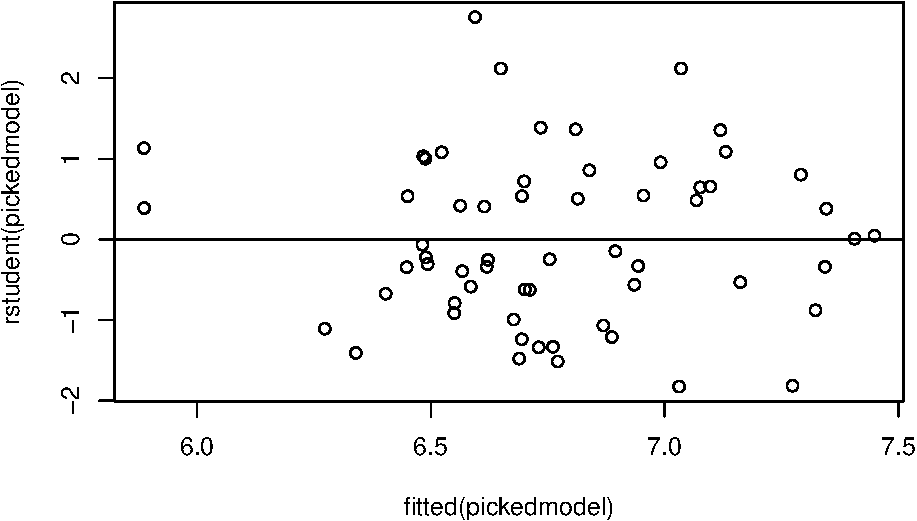
\includegraphics[keepaspectratio]{report_files/report_files/figure-latex/unnamed-chunk-33-1.pdf}}

Once again, very similar res vs fitted values as previous.

\begin{Shaded}
\begin{Highlighting}[]
\FunctionTok{qqnorm}\NormalTok{(}\FunctionTok{rstudent}\NormalTok{(pickedmodel)); }\FunctionTok{qqline}\NormalTok{(}\FunctionTok{rstudent}\NormalTok{(pickedmodel))}
\end{Highlighting}
\end{Shaded}

\pandocbounded{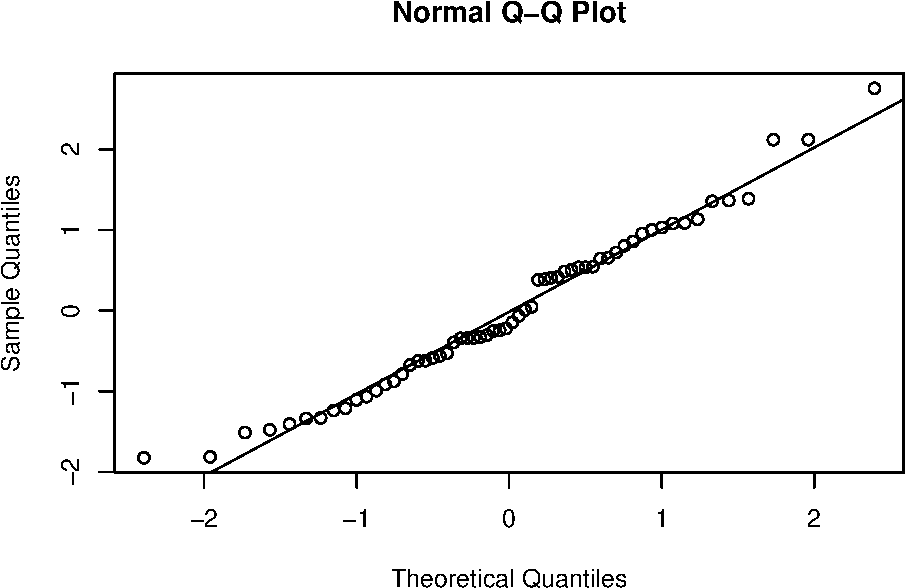
\includegraphics[keepaspectratio]{report_files/report_files/figure-latex/unnamed-chunk-34-1.pdf}}

Very close to normal distribution, still with a little light of tails,
though.

\subsubsection{g)}\label{g}

\begin{Shaded}
\begin{Highlighting}[]
\NormalTok{new\_lnx }\OtherTok{\textless{}{-}} \FunctionTok{data.frame}\NormalTok{(}\AttributeTok{x6=}\DecValTok{3100}\NormalTok{,}\AttributeTok{x7=}\FloatTok{2.1}\NormalTok{,}\AttributeTok{x8=}\FloatTok{1.1}\NormalTok{)}
\FunctionTok{exp}\NormalTok{(}\FunctionTok{predict}\NormalTok{(pickedmodel,new\_lnx,}\AttributeTok{interval=}\StringTok{\textquotesingle{}prediction\textquotesingle{}}\NormalTok{,}\AttributeTok{level=}\NormalTok{.}\DecValTok{95}\NormalTok{))}
\end{Highlighting}
\end{Shaded}

\begin{verbatim}
##        fit      lwr      upr
## 1 524.4452 190.5552 1443.376
\end{verbatim}

with a compensation of 1.5 million, we can now conclude that the ceo is
being paid a little too much, given our model, and what we expected. As
for the interval, it is tigher than the previous, as shown here:

\begin{Shaded}
\begin{Highlighting}[]
\NormalTok{new\_x }\OtherTok{\textless{}{-}} \FunctionTok{data.frame}\NormalTok{(}\AttributeTok{x1=}\DecValTok{48}\NormalTok{,}\AttributeTok{x2=}\DecValTok{1}\NormalTok{,}\AttributeTok{x4=}\DecValTok{14}\NormalTok{,}\AttributeTok{x5=}\DecValTok{3}\NormalTok{,}\AttributeTok{x6=}\DecValTok{3100}\NormalTok{,}\AttributeTok{x7=}\FloatTok{2.1}\NormalTok{,}\AttributeTok{x8=}\FloatTok{1.1}\NormalTok{,}\AttributeTok{x9=}\DecValTok{172}\NormalTok{)}
\FunctionTok{predict}\NormalTok{(redmodel,new\_x,}\AttributeTok{interval=}\StringTok{\textquotesingle{}prediction\textquotesingle{}}\NormalTok{,}\AttributeTok{level=}\NormalTok{.}\DecValTok{95}\NormalTok{)}
\end{Highlighting}
\end{Shaded}

\begin{verbatim}
##        fit       lwr      upr
## 1 761.5257 -268.8854 1791.937
\end{verbatim}

So we went from a width of around 2000, to a width of around 1200, which
is certainly a increase in certainty.

\end{document}
